% template.tex
% 
% This is a template for LaTeX's Beamer class.
%
% -----------------------------------------------------------------------------------
% Copyright (c) 2022 Masaki Tanaka (Washington University in St Louis)
% All rights researved.
%
% This source code or any portion thereof must not be reproduced or used
% in any manner whatsoever.
%
%

% ====================================================================================
%  1. Load Packages and Set Document Configurations
% ====================================================================================

\documentclass[
	11pt, % default font size (8pt, 9pt, 10pt, 11pt, 12pt, 14pt, 17pt, 20pt)
	%t,   % Uncomment to vertically align all slide content to the top of the slide, rather than the default centered
	%aspectratio=169, % If uncomment, aspect ratio is set to 16:9
]{beamer}

\graphicspath{{figs/}{./}} % directory containing the figures (trailing slash required)

\usepackage{booktabs} % Allows the use of \toprule, \midrule and \bottomrule for better rules in tables

% ----------------------------------------------------------------------------------------
%  1-1. Select a Beamer theme
% ----------------------------------------------------------------------------------------
% Following are the popular preset themes. Uncomment the one you want to use.
% For the detail of each theme, see https://deic.uab.cat/~iblanes/beamer_gallery/index_by_theme.html

%\usetheme{default}
%\usetheme{AnnArbor}
%\usetheme{Antibes}
%\usetheme{Bergen}
%\usetheme{Berkeley}
%\usetheme{Berlin}
%\usetheme{Boadilla}
%\usetheme{CambridgeUS}
%\usetheme{Copenhagen}
%\usetheme{Darmstadt}
%\usetheme{Dresden}
%\usetheme{Frankfurt}
%\usetheme{Goettingen}
\usetheme{Hannover}
%\usetheme{Ilmenau}
%\usetheme{JuanLesPins}
%\usetheme{Luebeck}
%\usetheme{Madrid}
%\usetheme{Malmoe}
%\usetheme{Marburg}
%\usetheme{Montpellier}
%\usetheme{PaloAlto}
%\usetheme{Pittsburgh}
%\usetheme{Rochester}
%\usetheme{Singapore}
%\usetheme{Szeged}
%\usetheme{Warsaw}

% ----------------------------------------------------------------------------------------
%  1-2. Select a color profile
% ----------------------------------------------------------------------------------------
% Following are the popular preset color profiles. Uncomment the one you want to use.
% For the detail of each profile, see https://deic.uab.cat/~iblanes/beamer_gallery/index_by_color.html

\usecolortheme{default}
%\usecolortheme{albatross}
%\usecolortheme{beaver}
%\usecolortheme{beetle}
%\usecolortheme{crane}
%\usecolortheme{dolphin}
%\usecolortheme{dove}
%\usecolortheme{fly}
%\usecolortheme{lily}
%\usecolortheme{monarca}
%\usecolortheme{seagull}
%\usecolortheme{seahorse}
%\usecolortheme{spruce}
%\usecolortheme{whale}
%\usecolortheme{wolverine}

% ----------------------------------------------------------------------------------------
%  1-3. Select a font theme
% ----------------------------------------------------------------------------------------
% Following are the preset font themes. Uncomment the one you want to use.
% For the detail of each profile, see https://deic.uab.cat/~iblanes/beamer_gallery/index_by_font.html

\usefonttheme{default} % Default sans serif font
%\usefonttheme{serif}  % Default serif font

%\usefonttheme{structurebold} % Make structure texts (e.g. titles, headlines) bold
%\usefonttheme{structureitalicserif} % Make structure texts italic serif
%\usefonttheme{structuresmallcapsserif} % Make structure texts small caps serif

%----------------------------------------------------------------------------------------
%  1-4.	SELECT OUTER THEME
%----------------------------------------------------------------------------------------

% Outer themes change the overall layout of slides, such as: header and footer lines, sidebars and slide titles. Uncomment each theme in turn to see what changes it makes to your presentation.

\useoutertheme{default}
%\useoutertheme{infolines}
%\useoutertheme{miniframes}
%\useoutertheme{smoothbars}
%\useoutertheme{sidebar}
%\useoutertheme{split}
%\useoutertheme{shadow}
%\useoutertheme{tree}
%\useoutertheme{smoothtree}

%\setbeamertemplate{footline} % Uncomment this line to remove the footer line in all slides

%\setbeamertemplate{footline}[page number] % Uncomment this line to replace the footer line in all slides with a simple slide count

%\setbeamertemplate{navigation symbols}{} % Uncomment this line to remove the navigation symbols from the bottom of all slides

%----------------------------------------------------------------------------------------
%  1-5.	SELECT INNER THEME
%----------------------------------------------------------------------------------------

% Inner themes change the styling of internal slide elements, for example: bullet points, blocks, bibliography entries, title pages, theorems, etc. Uncomment each theme in turn to see what changes it makes to your presentation.

\useinnertheme{default}
%\useinnertheme{circles}
%\useinnertheme{rectangles}
%\useinnertheme{rounded}
%\useinnertheme{inmargin}



% ====================================================================================
%  2. Set Presentation Information
% ====================================================================================

% Presentation Title
\title[Short Title]{Full Presentation Title}
%\title{Full Presentation Title}

% Presentation subtitle
% Uncomment the following line if no subtitle
\subtitle{Subtitle (Optional)} 

% Presenter name(s)
\author[Author1 \and Author2]{First Author \and Second Author}
%\author{First Author \and Second Author}

% Affiliation(s)
\institute[WUSTL]{Washington University in St. Louis \\ \smallskip \textit{corresponding.author@wustl.edu}}
%\institute{Washington University in St. Louis \\ \smallskip \textit{corresponding.author@wustl.edu}}

% Presentation date and conference/meeting name
\date[\today]{Macroeconomics Workshop \\ \today}
%\date{Beamer Workshop \\ \today}




% ====================================================================================
%  3. Contents of Presentation
% ====================================================================================

\begin{document}

%----------------------------------------------------------------------------------------
%  3-1) Title page
%----------------------------------------------------------------------------------------
\begin{frame}
	\titlepage % This command automatically generates the tile page based on the presentation information
\end{frame}

%----------------------------------------------------------------------------------------
%  3-2) Agenda
%----------------------------------------------------------------------------------------
\begin{frame}
	\frametitle{Agenda} % Slide title. Uncommemnt if no title
	
	\tableofcontents % This command automatically generates the table of contents, using the names of sections and subsections declared later
\end{frame}

%----------------------------------------------------------------------------------------
%  3-3) Body slides
%----------------------------------------------------------------------------------------
\section{Section I} % Section Name

%........................................................................................
\subsection{Subsecrtion 1} % Subsection Name

% Body slide 1
\begin{frame}
	\frametitle{Body slide example 1} % Slide title. Uncommemnt if no title
	\framesubtitle{Motivation}  % Slide subtitle. Uncommemnt if no subtitle
	
	\begin{itemize}
		\item After the outbreak of COVID-19, the global economy experienced ...
		\item The literature has yet to identify its causes.
		\begin{itemize}
			\item A survey conducted by World Bank implies ....
			\item However, the recent survey by IMF shows ...
		\end{itemize}
		\item Three possible causes:
		\begin{enumerate}
			\item Item 1
			\item Item 2
			\item Item 3 
		\end{enumerate}
	\end{itemize}
\end{frame}

% Body slide 2
\begin{frame}
	\frametitle{Body slide example 2} % Slide title. Uncommemnt if no title
	\framesubtitle{What we do}  % Slide subtitle. Uncommemnt if no subtitle
	\begin{enumerate}
		\item Construct a general equilibrium model incorporating ... 
		\item Take the model to the data including the pandemic period.
		\item Run simulations with the estimated model.
	\end{enumerate}
\end{frame}

% Body slide 3
\begin{frame}
	\frametitle{Body slide example 3} % Slide title. Uncommemnt if no title
	\framesubtitle{What we find}  % Slide subtitle. Uncommemnt if no subtitle
	
	\begin{itemize}
		\item Our findings are threefold:
		\begin{enumerate}
			\item Finding 1
			\item Finding 2
			\item Finding 3
		\end{enumerate}
	\end{itemize}
	
	\bigskip % Vertical blankspace
	
	\begin{itemize}
		\item Additional Comment 1
		\item Additional Comment 2
	\end{itemize}
\end{frame}

%........................................................................................
\subsection{Subsecrtion 2} % Subsection Name

% Body slide 4
\begin{frame}
	\frametitle{Blocks of Highlighted Text}
	
	\begin{block}{Block Title}
		``block'' generates this type of block.
	\end{block}
	
	\begin{exampleblock}{Example Block Title}
		``exampleblock'' generates this type of block.
	\end{exampleblock}
	
	\begin{alertblock}{Alert Block Title}
		``alertblock'' generates this type of block.
	\end{alertblock}
	
	\begin{block}{} % Block without title
		You can use these commends without a title. If you do so,
		this type of block will be generated.
	\end{block}
\end{frame}

% Body slide 5
\begin{frame}
	\frametitle{Definitions \& Theorem}
	
	\begin{definition}
		A good is \alert{normal} if the demand for it increases as income rises.
	\end{definition}

	\bigskip % Vertical whitespace

	\begin{theorem}[1st Fundermental Theorem of Welfare Economies]
		If the price and allocation constitute a competitive equiolibrium, then
		this allocation is Pareto optimal.
	\end{theorem}
\end{frame}

% Body slide 6
\begin{frame}
	\frametitle{Lemma, Proof, \& Corollary}
	
	\begin{lemma}[Shepard's lemma]
		If $z(\bar{w}, q)$ consists of a single point, then $c(\cdot)$ is differentiable
		with respect to $w$ at $\bar{w}$ and $\nabla_{w} c(\bar{w}, q) = z(\bar{w}, q)$.
	\end{lemma}

	\begin{proof}
		See Chapter 15 of the textbook.
	\end{proof}

	\bigskip % Vertical whitespace

	\begin{corollary}
		A pure strategy profile is a Nash equilibrium of a game if and only if it is
		a degenerated mixed-strategy Nash equilibrium of the game.
	\end{corollary}
\end{frame}

%-----------------------------------------------------------------------------------------
\section{Section II}

%........................................................................................
\subsection{Example Table}

% Body slide 7
\begin{frame}
	\frametitle{Table}
	\framesubtitle{How to include tables} % Optional subtitle
	
	\begin{table}
		\begin{tabular}{l l l}
			\toprule
			\textbf{Parameter} & \textbf{Value} & \textbf{S.E.}\\
			\midrule
			Parameter 1 & 3.443 & 0.562 \\
			Parameter 2 & 2.110 & 0.910 \\
			Parameter 3 & 0.310 & 0.096 \\
			\bottomrule
		\end{tabular}
		\caption{Table caption}
	\end{table}
\end{frame}

%........................................................................................
\subsection{Example Figure}

% Body slide 8
\begin{frame}
	\frametitle{Figure}
	\framesubtitle{How to include figures} % Optional subtitle
	
	\begin{figure}
		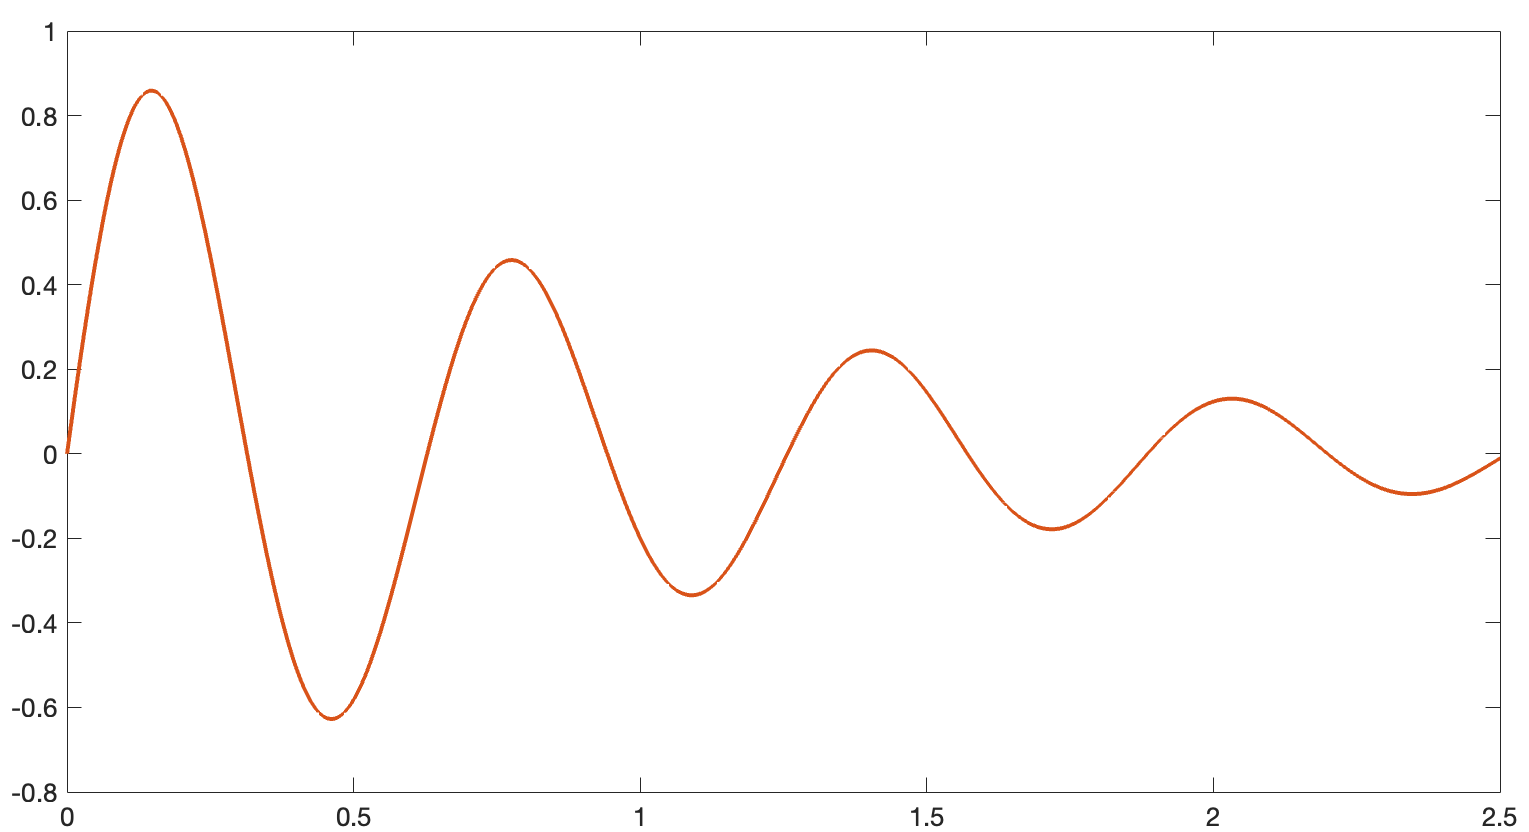
\includegraphics[width=0.95\linewidth]{sample_fig.png}
		\caption{Figure Caption}
	\end{figure}
\end{frame}


%-----------------------------------------------------------------------------------------
\section{Section III}

% Body slide 9
\begin{frame}
	\frametitle{Equation}

	\begin{equation}
		i_{t} = i^{*} + \phi_{y} (y_{t} - y^{*}) + \phi_{\pi} (\pi_{t} - \pi^{*})
	\end{equation}
\end{frame}

% Body slide 10
\begin{frame}[fragile] % Need to use the fragile option when verbatim is used in the slide
	\frametitle{Verbatim}
	
	\begin{example}[Figure Slide Code]
		\footnotesize % Reduce the font size only in this "example block"
		\begin{verbatim}
			\begin{figure}
				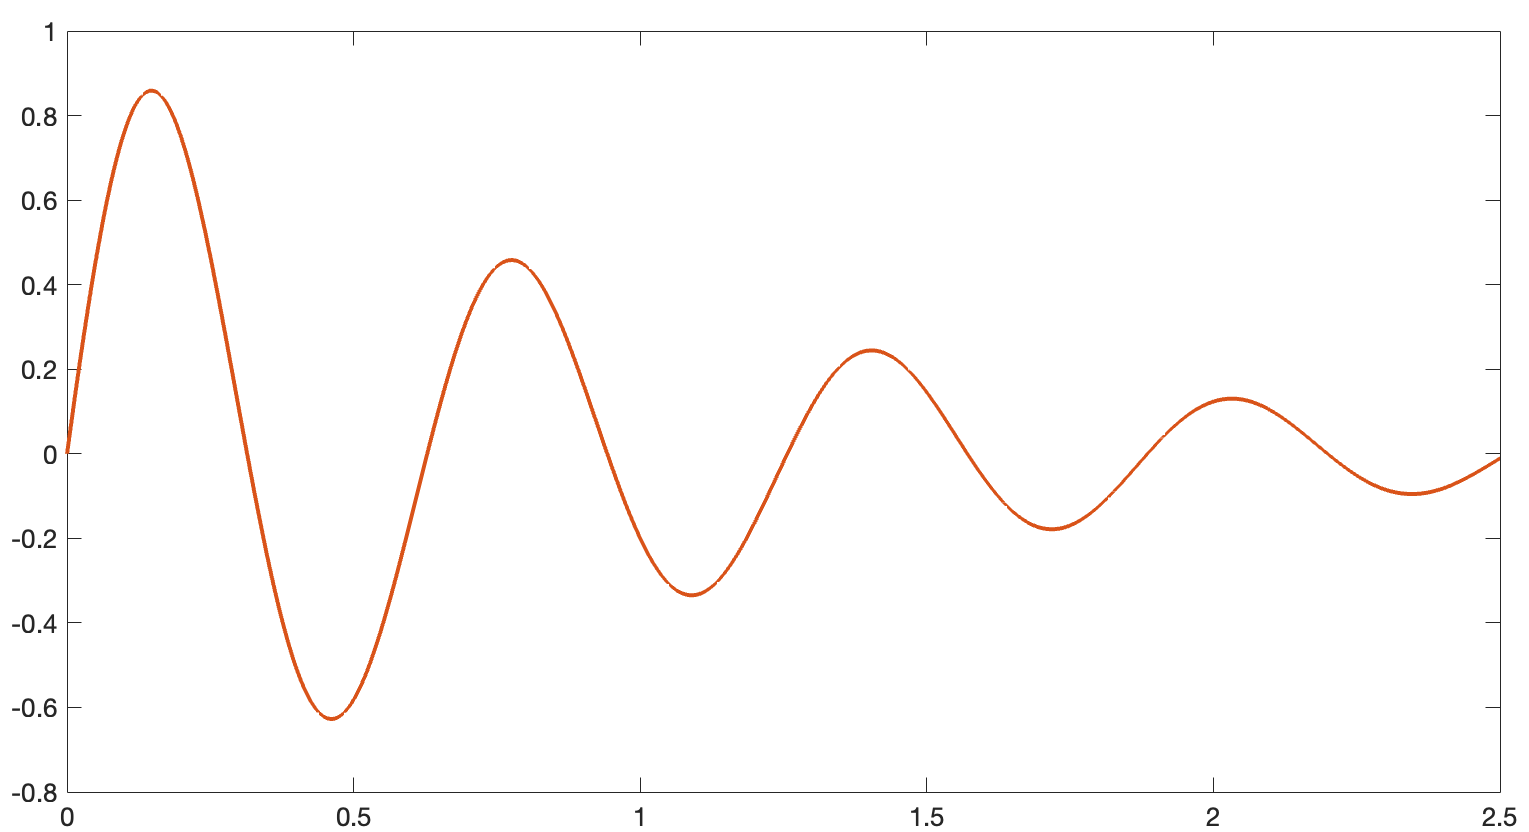
\includegraphics[width=0.95\linewidth]{sample_fig.png}
				\caption{Figure Caption}
			\end{figure}\end{verbatim} % Must be on the same line
	\end{example}
\end{frame}

% Body slide 11
\begin{frame}
	Slide without title.
\end{frame}

%-----------------------------------------------------------------------------------------
% Body slide 12
\section{Section IV}

\begin{frame}
	\frametitle{Citing References}

	\begin{itemize}
		\item Literature focuses on
		\begin{enumerate}
			\item imperfect information \cite{ref1}
			\item transaction cost \cite{ref2}
		\end{enumerate}
		\item This is an example of citing references.
	\end{itemize}
\end{frame}

%-----------------------------------------------------------------------------------------

\begin{frame} % Use [allowframebreaks] to allow automatic splitting across slides if the reference list is too long
	\frametitle{References}
	
	\begin{thebibliography}{99} 
		% Beamer does not support BibTeX. Thus, you have to write references by yourself.
		\footnotesize % Reduce the font size in the reference section
		
		\bibitem[Smith, 2022]{ref1}
			John Smith (2022)
			\newblock ``People buy what, when, and why?''
			\newblock \emph{Example Journal of Economic Theory} 1(3), 445 -- 487.
			
		\bibitem[Appleseed, 2020]{ref2}
			Jane Appleseed (2020)
			\newblock ``Invest less and consume less''
			\newblock \emph{Microeconomics and Macroeconomics} 22(1), 19 -- 48.
	\end{thebibliography}
\end{frame}

%----------------------------------------------------------------------------------------

\end{document} 